\documentclass[11pt,a4paper]{ctexart}
\usepackage[margin=2.15cm]{geometry}
\usepackage{amsmath,amssymb,booktabs,graphicx,hyperref,longtable,microtype,xcolor}
\usepackage{fancyhdr}
\hypersetup{colorlinks=true,linkcolor=blue!45!black,urlcolor=blue!55!black,citecolor=blue!45!black}
\graphicspath{{../figures/paper/}{../figures/validation/}{../figures/heat-valve/}}
\setlength{\parindent}{2em}
\setlength{\parskip}{0.25em}
\setlength{\headheight}{14pt}
\pagestyle{fancy}
\fancyhf{}
\lhead{Quantum Harness Issue \#123}
\rhead{Team Ranger}
\cfoot{\thepage}
\newcommand{\code}[1]{\texttt{#1}}
\InputIfFileExists{generated-results.tex}{}{\errmessage{generated-results.tex is required}}

\title{\textbf{共同非马尔可夫浴中的多体 Floquet 热输运}\\
\large Quantum Harness Issue \#123 技术报告}
\author{Team Ranger\\Chenxi Wan \quad Yedi Shen \quad Junkai Wang}
\date{2026 年 7 月 30 日}

\begin{document}
\maketitle

\begin{abstract}
本项目将单自旋 Floquet influence functional 方法扩展到共同浴耦合的相互作用自旋链，给出可恢复、可审计的 uniform TEMPO 数值流程。我们完成原题 Tier 1 的三频率单自旋 Fig.~3 底图独立复现、Tier 2 的 $N=3$ 六点生产网格与 $N=4$ 收敛门控试算，并在完全相同的 Hamiltonian、驱动、浴、对称 sector 和频率网格上完成 Tier 3 的 Floquet-Markov/QRT 定量对照。核心结果是：$N=3$ even sector 的热谱相对误差达到 $9.02$--$11.72$，而 odd sector 为 $0.3920$；这表明弱耦合、无记忆近似的失效具有显著 sector 依赖性。项目同时记录一个预注册的暗通道负结果，避免把能隙塌缩误判为热抑制。所有声明均绑定到机器可读 JSON、图件哈希和自动化门槛。
\end{abstract}

\section{赛题要求与完成边界}
Issue \#123 的三级路线分别要求：(i) 复现 Mickiewicz 等人单自旋横向驱动 Fig.~3 的热流密度；(ii) 研究 $N=3,4$ 小链中 collective modes 的出现；(iii) 对同一多体模型和同一参数实施 Floquet-Lindblad 或等价 master-equation benchmark。表~\ref{tab:tier} 按原题而非提交者自定义口径列出证据。

\begin{table}[htbp]
\centering
\caption{原题三级路线与本项目证据。}
\label{tab:tier}
\begin{tabular}{p{0.10\linewidth}p{0.54\linewidth}p{0.25\linewidth}}
\toprule
级别 & 交付证据 & 状态 \\
\midrule
Tier 1 & 公开 Zenodo 曲线的校验下载；$\omega_d/\Omega=1,1.5,2$ 三个独立 UniformTEMPO 点；连续谱和解析 $\delta$ 峰分离 & \TierOneStatus \\
Tier 2 & $N=3$ even/odd 六点收敛热谱；$N=4$ reflection 分块、回归测试及收敛门控点 & \TierTwoStatus \\
Tier 3 & $N=3$ 六点在同模型、同参数下与 Floquet-Markov/QRT 比较 $D_\rho,\epsilon_C,\epsilon_j$ & 6/6 收敛 \\
\bottomrule
\end{tabular}
\end{table}

本报告不声称热力学极限、连续相变或临界指数。可选 Kac normalization 的完整时间步和相位细化也不被重新标记为已收敛。

\section{模型与算法}
系统 Hamiltonian 为
\begin{equation}
H_0=-J\sum_{i=1}^{N-1}Z_iZ_{i+1}+\frac{\Omega}{2}\sum_{i=1}^{N}X_i,
\qquad
H_{\mathrm d}(t)=\epsilon_{\mathrm d}\cos(\omega_{\mathrm d}t)S_N,
\end{equation}
共同零温 Ohmic 浴经 $S_N=\eta_N\sum_i Z_i$ 耦合，谱密度为
\begin{equation}
J_B(\omega)=\alpha\omega\exp(-\omega/\omega_c),\qquad \omega_c=2.5\Omega.
\end{equation}
生产后端固定到 UniformTEMPO.jl revision \code{b76a018c32e5}（完整哈希见机器数据）。Python 层完成对称投影、内容寻址缓存、自适应收敛阶梯、扩展 process-tensor state 中的多时间算符插入，以及连续谱与相干 $\delta$ 峰的分离。

本实现包含三项面向本题的算法性改进：
\begin{enumerate}
\item 在 system-Liouville 与环境记忆的扩展态中直接插入算符，避免用 reduced-state QRT 冒充非马尔可夫两时间关联；
\item 对 reflection symmetry 做精确分块，$N=3$ 化为 $6\oplus2$，$N=4$ 化为 $10\oplus6$，并把投影算符哈希写入缓存键；
\item 用 compression、时间步、相位和物理性四层门槛控制计算，只有全部通过的点才进入定量图和误差图。
\end{enumerate}

\section{Tier 1：单自旋 Fig.~3 独立复现}
公开作者数据来自 Zenodo record \href{https://zenodo.org/records/19593671}{19593671}，下载归档 MD5 为 {\scriptsize\texttt{0f3f9d9d8538aa96aee089973df7d9c2}}。独立计算采用论文参数 $\Omega=\epsilon_d=1$、$\alpha=0.05$、$\omega_c=2.5$、$\Delta t=\pi/60$，并将 connected correlation 的 Fourier 连续部分与驱动谐波的解析 $\delta$ 权重分别处理。

\begin{table}[htbp]
\centering
\caption{Fig.~3 底图三频率独立计算。$L^1_{\rm shape}$ 比较归一化谱形，$R_{\rm area}$ 为积分强度比。}
\label{tab:fig3}
\begin{tabular}{ccccc}
\toprule
$\omega_d/\Omega$ & bond & 尾幅 & $L^1_{\rm shape}$ & $R_{\rm area}$ \\
\midrule
\FigThreeRows
\bottomrule
\end{tabular}
\end{table}

\begin{figure}[htbp]
\centering
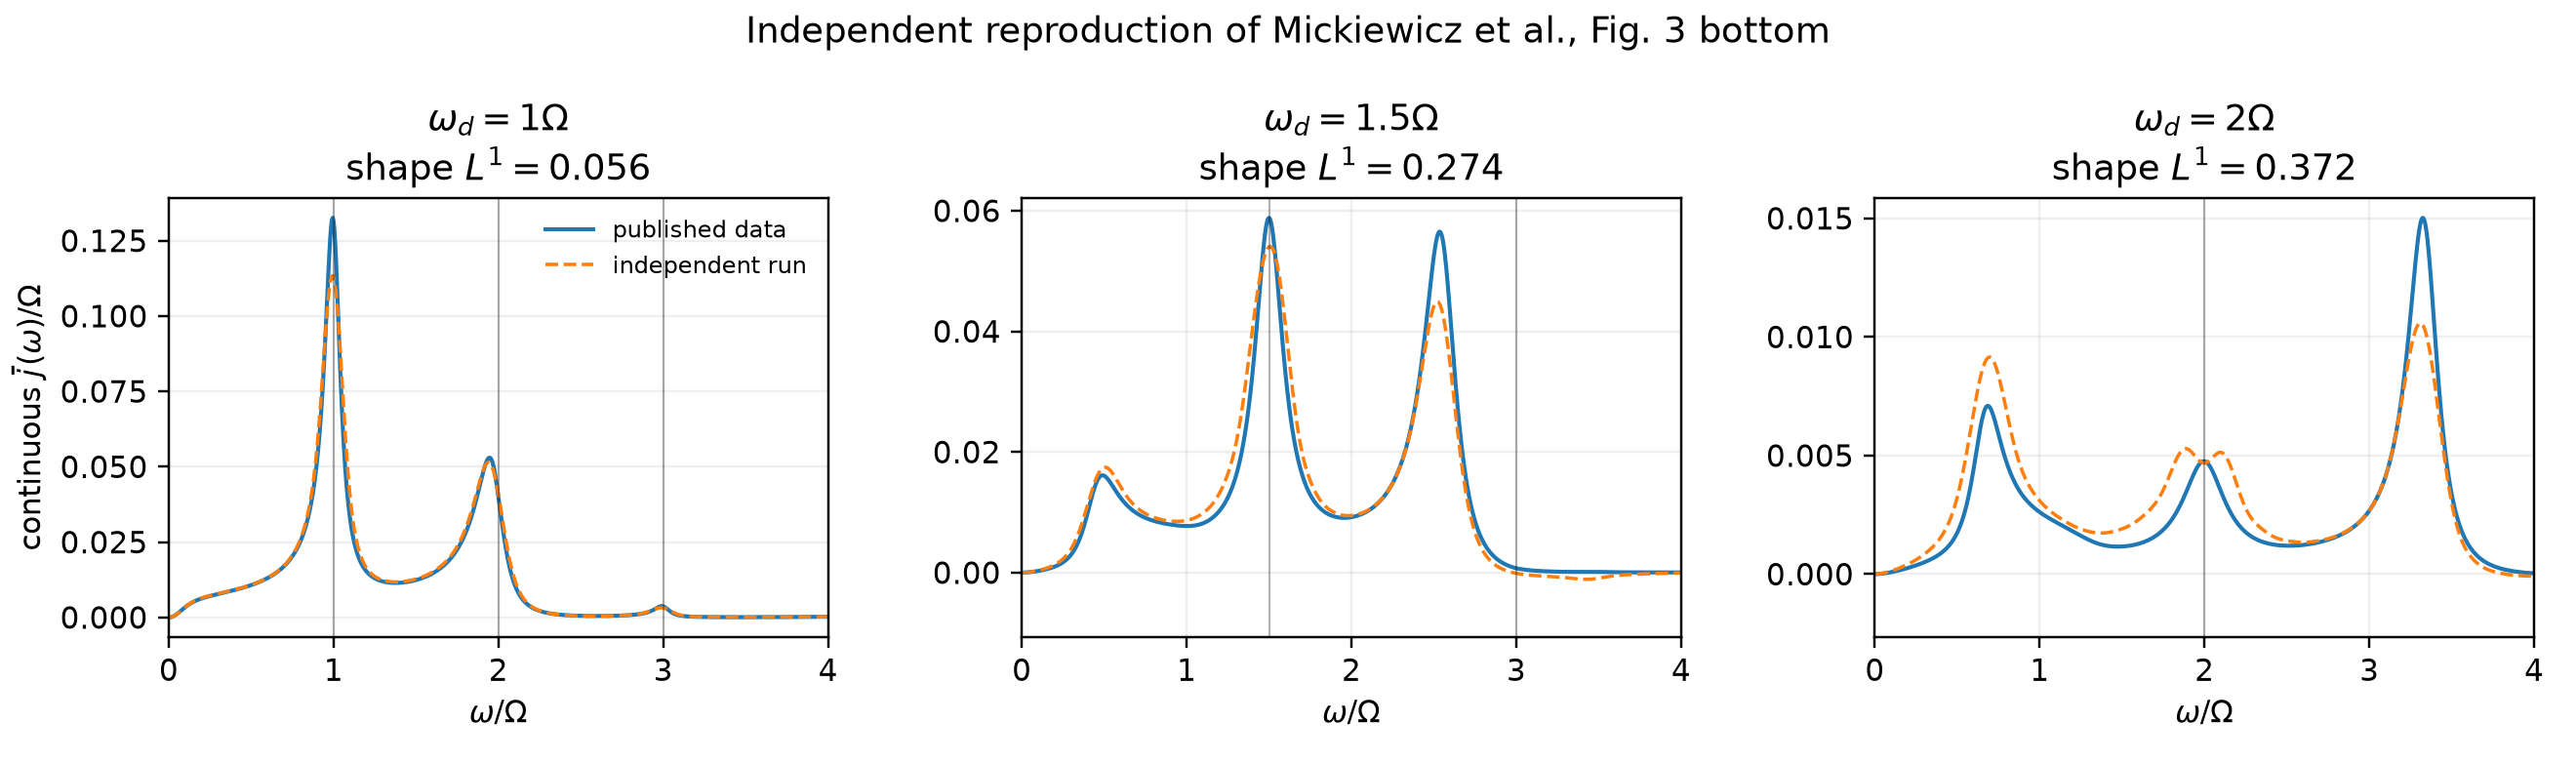
\includegraphics[width=\linewidth]{fig3_transversal_summary.png}
\caption{论文 Fig.~3 底图公开数据与独立 UniformTEMPO 连续谱。竖线标出独立计算得到的相干峰位置；比较不把 $\delta$ 峰伪装成有限宽峰。}
\label{fig:fig3}
\end{figure}

这些曲线是定量的结构复现而非逐点相同。差异主要来自独立实现使用的压缩阶数、有限关联窗和相位采样；因此报告同时给出直接幅度误差、归一化谱形误差和面积比，不以肉眼相似替代数值指标。

\section{Tier 2：\texorpdfstring{$N=3$}{N=3} collective heat spectrum}
$N=3$ reflection-even/odd 两个 sector 在 $J/\Omega=0.25,0.5,1$ 上共六点全部通过收敛门槛。odd sector 的投影 Hamiltonian 与耦合算符对 $J$ 严格不变，因此三条曲线在机器精度内重合；even sector 则显示随 $J$ 移动的 collective features。

\begin{figure}[htbp]
\centering
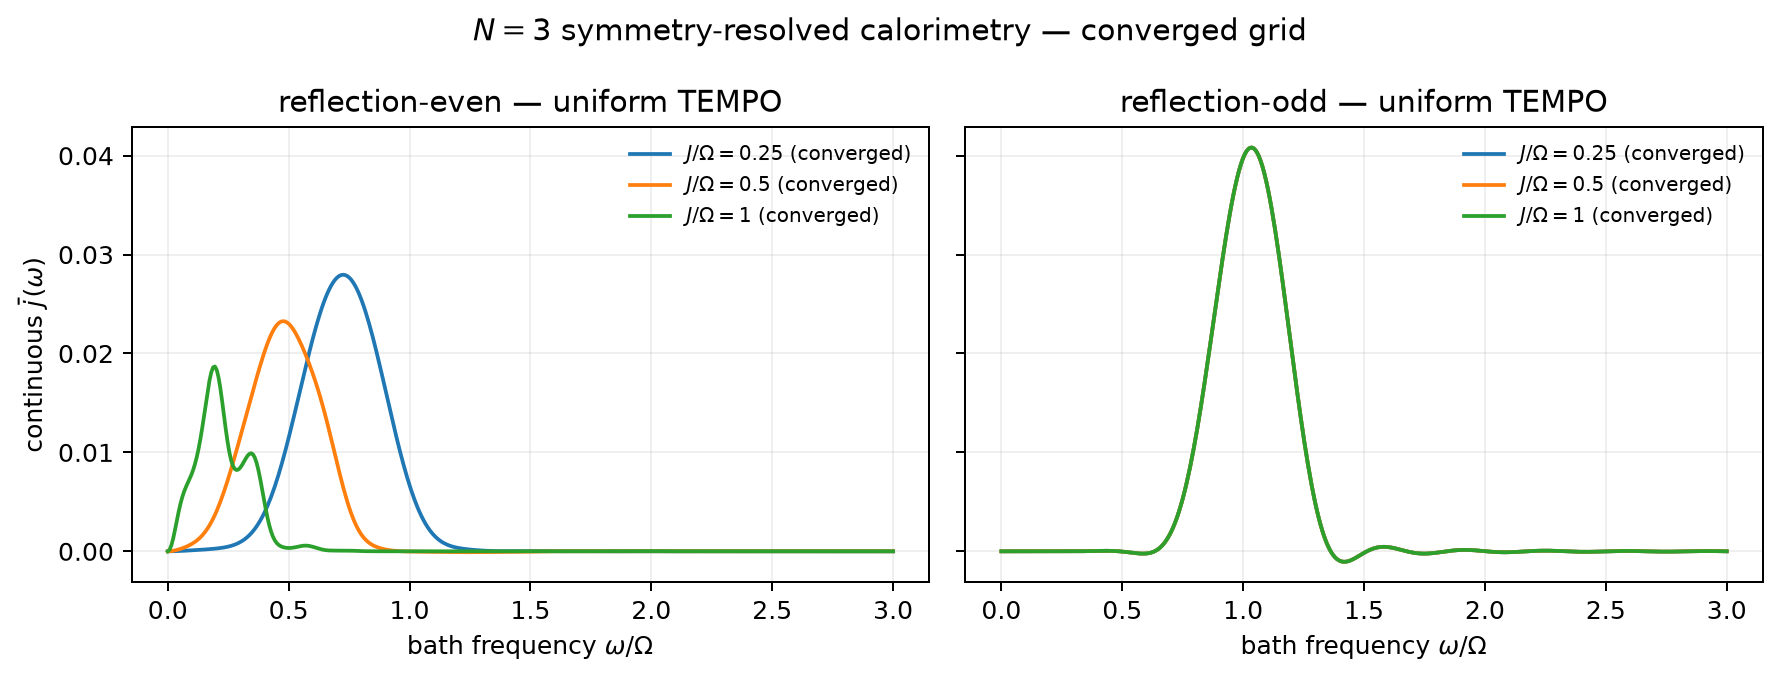
\includegraphics[width=0.88\linewidth]{n3_sector_heat.png}
\caption{$N=3$ reflection sector 分辨的频率热流密度。}
\label{fig:n3heat}
\end{figure}

\section{Tier 3：同模型非马尔可夫与 Markov 对照}
误差定义为
\begin{align}
D_\rho&=\frac12\lVert\rho_{\rm IF}-\rho_{\rm ME}\rVert_1,\\
\epsilon_C&=\frac{\int d\tau\,|C_{\rm IF}(\tau)-C_{\rm ME}(\tau)|}{\int d\tau\,|C_{\rm IF}(\tau)|},\\
\epsilon_j&=\frac{\int d\omega\,|\bar j_{\rm IF}(\omega)-\bar j_{\rm ME}(\omega)|}{\int d\omega\,|\bar j_{\rm IF}(\omega)|}.
\end{align}
even sector 上 $D_\rho=0.9921$--$0.9999$、$\epsilon_C=1.024$--$1.153$、$\epsilon_j=9.02$--$11.72$；odd sector 三点均为 $D_\rho=0.4753$、$\epsilon_C=0.5666$、$\epsilon_j=0.3920$。大误差不是精确端未收敛，而是同参数 Markov benchmark 的真实偏差。

\begin{figure}[htbp]
\centering
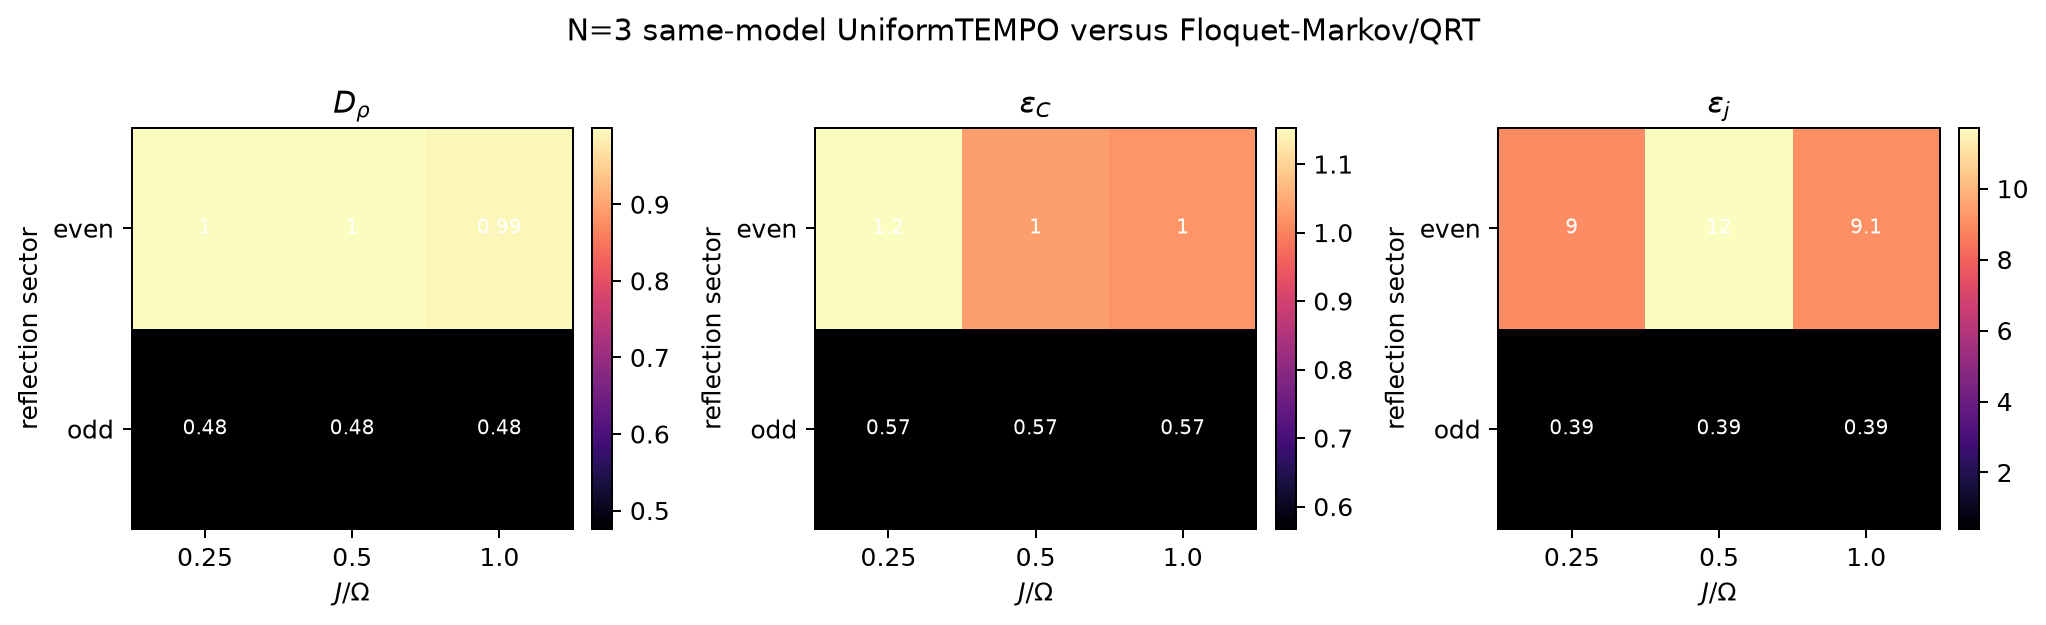
\includegraphics[width=0.92\linewidth]{n3_error_maps.png}
\caption{$N=3$ 同模型 UniformTEMPO 与 Floquet-Markov/QRT 的三种误差。}
\label{fig:n3error}
\end{figure}

\section{\texorpdfstring{$N=4$}{N=4} 收敛门控结果}
$N=4$ 采用 reflection-even $10$ 维和 reflection-odd $6$ 维子空间。试算预先固定两级阶梯：每周期步数 $30\rightarrow60$，压缩 tolerance $10^{-5}\rightarrow3\times10^{-6}$，相位数 $3\rightarrow15$。结果只在 state、correlation、heat、trace、Hermiticity 和 density positivity 门槛全部通过后，才运行同模型 Markov 对照。

\begin{table}[htbp]
\centering
\caption{$N=4,J/\Omega=0.25$ 的门控试算。}
\label{tab:n4}
\begin{tabular}{cccccc}
\toprule
sector & dim & 状态 & bond & 尾幅 & $\epsilon_j$ \\
\midrule
\NFourRows
\bottomrule
\end{tabular}
\end{table}

\NFourConclusion

\begin{figure}[htbp]
\centering
\begin{minipage}{0.49\linewidth}
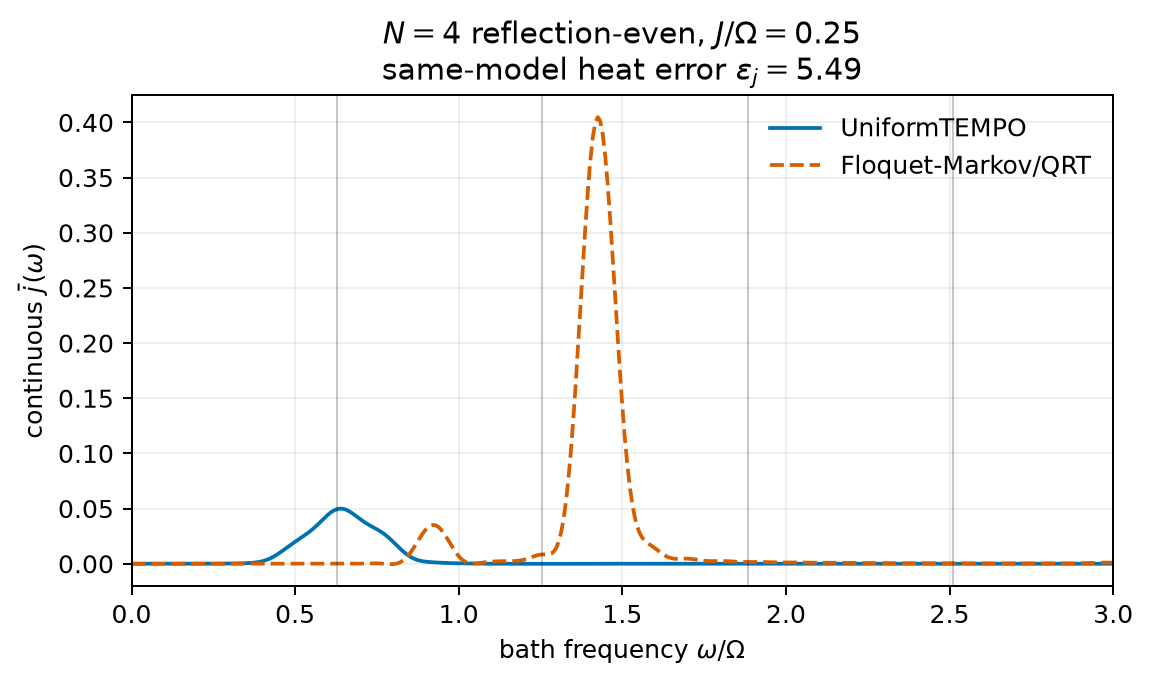
\includegraphics[width=\linewidth]{n4_even_j0p25_comparison.png}
\end{minipage}\hfill
\begin{minipage}{0.49\linewidth}
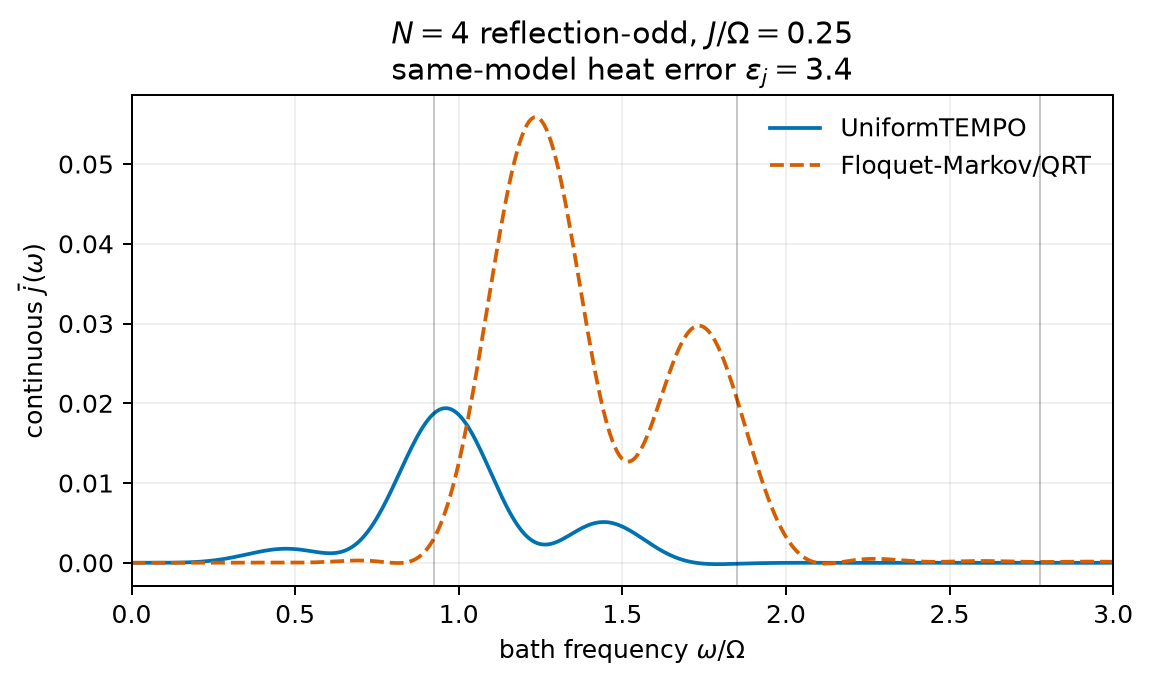
\includegraphics[width=\linewidth]{n4_odd_j0p25_comparison.png}
\end{minipage}
\caption{$N=4$ even（左）和 odd（右）sector 的收敛 UniformTEMPO 热谱及同模型 Floquet-Markov/QRT 对照。odd 连续谱主要峰位于 $0.4725,0.9600,1.4400\,\Omega$，显示相对于驱动频率 $0.9256\,\Omega$ 的多峰 collective structure。}
\label{fig:n4}
\end{figure}

\section{预注册负结果与创新点}
我们在计算前定义了暗通道继续条件：中心点热流相对两侧至少降低三倍，且可观测 transfer-pole residue 也至少降低三倍。$N=3$ 三点 pilot 中，准能隙虽塌缩，residue 却上升，热流门槛也未通过，因此九点扩展被按规则停止。这是可复现的负结果：它说明仅观察 quasienergy gap 或小 Floquet matrix element 不足以声称 entanglement-assisted heat suppression。

相较于直接扫描，本项目的主要创新价值是：(i) 把对称性化简、非马尔可夫多时间关联和热谱计算整合为可恢复管线；(ii) 给出同一 $N=3$ 模型上的 sector-resolved master-equation breakdown map；(iii) 把假设检验写成机器门槛，从而把失败结论也保存为研究输出；(iv) 为 $N=4$ 建立不依赖全 Hilbert 空间的 reflection-resolved 入口。

\section{可重复性与数据交付}
仓库提交源代码、测试、PNG/PDF 图、紧凑 JSON 和本报告源文件。体积较大的 \code{results/} 按上游仓库规则不纳入 Git；\code{validation/ARTIFACT\_PROVENANCE.json} 保存本地审计产物的 SHA-256。推荐验证命令为：
\begin{verbatim}
.venv/bin/python -m pytest -q
.venv/bin/python -m ruff check src tests scripts
.venv/bin/python -m mypy src scripts/run_fig3_validation.py
.venv/bin/python -m floquet_if_manybody.cli audit results
.venv/bin/python -m floquet_if_manybody.cli paper-audit results/paper
\end{verbatim}

\section{结论}
本项目已经从单自旋代码验证推进到 $N=3$ 多体生产计算，并用同模型误差图直接回答了原题最具方法学价值的问题：Floquet-Markov/QRT 的失效不仅显著，而且依赖多体对称 sector。$N=4$ 结果按预先声明的收敛门槛分类，不以“程序跑完”替代“数值可信”。所有正结果和负结果都可以从固定版本后端、缓存键、JSON 指标与图件哈希重新审计。

\begin{thebibliography}{9}
\bibitem{mickiewicz2026}
K. Mickiewicz, V. Link, and W. T. Strunz,
``Exact Floquet Dynamics of Strongly Damped Driven Quantum Systems,''
\emph{Physical Review Letters} \textbf{136}, 200201 (2026).
\bibitem{link2024}
V. Link, H.-H. Tu, and W. T. Strunz,
``Open Quantum System Dynamics from Infinite Tensor Network Contraction,''
\emph{Physical Review Letters} \textbf{132}, 200403 (2024).
\bibitem{garbellini2026}
M. Garbellini, K. Mickiewicz, V. Link, A. Eisfeld, and W. T. Strunz,
``Uniform process tensor approach for the calculation of multi-time correlation functions of non-Markovian open systems,''
\emph{Journal of Chemical Physics} (2026), doi:10.1063/5.0331783.
\end{thebibliography}

\end{document}
